%%
%% prog-folien
%%
%% Slides for my Java programming tutorial using LaTeX beamer.
%%
%% Copyright (c) 2015-2016 YouniS Bensalah <younis.bensalah@riseup.net>
%%
%% This work is released to the public domain.
%% For the full copyright and license information, please view the LICENSE file.
%%

%% LaTeX-Beamer template for KIT design
%% by Erik Burger, Christian Hammer
%% title picture by Klaus Krogmann
%%
%% version 2.1
%%
%% mostly compatible to KIT corporate design v2.0
%% http://intranet.kit.edu/gestaltungsrichtlinien.php
%%
%% Problems, bugs and comments to
%% burger@kit.edu

\documentclass[18pt]{beamer}

%% SLIDE FORMAT

% use 'beamerthemekit' for standard 4:3 ratio
% for widescreen slides (16:9), use 'beamerthemekitwide'

\usepackage{templates/beamerthemekit}
% \usepackage{templates/beamerthemekitwide}

\usepackage[utf8]{inputenc}
\usepackage{hyperref}
\usepackage{listings}
%\usepackage{xcolor}
%\usepackage{colortbl}
%\usepackage{array}
%\usepackage{tikz}
%\usetikzlibrary{calc,shapes.multipart,chains,arrows}

%\definecolor{lime}{HTML}{8FFF53}

\newcommand{\quotes}[1]{``#1''}

%% TITLE PICTURE

% if a custom picture is to be used on the title page, copy it into the 'logos'
% directory, in the line below, replace 'mypicture' with the
% filename (without extension) and uncomment the following line
% (picture proportions: 63 : 20 for standard, 169 : 40 for wide
% *.eps format if you use latex+dvips+ps2pdf,
% *.jpg/*.png/*.pdf if you use pdflatex)

\titleimage{greendrop}

%% TITLE LOGO

% for a custom logo on the front page, copy your file into the 'logos'
% directory, insert the filename in the line below and uncomment it

%\titlelogo{mylogo}

% (*.eps format if you use latex+dvips+ps2pdf,
% *.jpg/*.png/*.pdf if you use pdflatex)

%% TikZ INTEGRATION

% use these packages for PCM symbols and UML classes
% \usepackage{templates/tikzkit}
% \usepackage{templates/tikzuml}

% the presentation starts here

\title[Generics]{Programmieren:\\ Generics}
\subtitle{Tutorium 30}
\author{YouniS Bensalah}
\date{December 11, 2015}

\institute{Chair for Software Design and Quality}

% Bibliography

\usepackage[citestyle=authoryear,bibstyle=numeric,hyperref,backend=biber]{biblatex}
\addbibresource{templates/example.bib}
\bibhang1em

\begin{document}

% change the following line to "ngerman" for German style date and logos
\selectlanguage{english}

%title page
\begin{frame}
\titlepage
\end{frame}

%table of contents
\begin{frame}{Heute}
\tableofcontents
\end{frame}

\section{Organisatorisches}

\begin{frame}{Termine}
    \textbf{Vorlesung}
    \begin{itemize}
        \item Die Vorlesung am 23.12.2015 entfällt.
        \item Die erste Vorlesung 2016 findet am 13.01.2016 statt.
    \end{itemize}

    \textbf{Tutorien}
    \begin{itemize}
        \item Die Tutorien finden im Jahr 2015 bis zum 22.12.2015 statt.
        \item Die Tutorien im Jahr 2016 beginnen ab dem 13.01.2016.
    \end{itemize}
\end{frame}


\begin{frame}{Checkstyle}
    \begin{itemize}
        \item Anzahl vorgegebener Regeln, die den Programmierer \quotes{zwingen}, sauberen und lesbaren Code zu schreiben
        \item Diese Regeln werden in einer Checkstyle-XML-Datei zusammengefasst und können automatisch überprüft werden
        \item Nicht nur der Compiler muss den Code verstehen !
        \item Gecheckt werden\dots
        \begin{itemize}
            \item Whitespaces
            \item Namenskonventionen
            \item JavaDoc
        \end{itemize}
        \item Siehe \textit{Checkstyle} in der \textit{Programmieren Wiki} im ILIAS\\
        \url{https://ilias.studium.kit.edu/goto.php?target=wiki_462045_Checkstyle}
    \end{itemize}

\end{frame}

\begin{frame}{Read the fine manual}
    \begin{itemize}
        \item \textbf{Programmieren-Wiki im ILIAS}
        \begin{itemize}
            \item \alert{Checkstyle}
            \item Programmierstil
            \item Javadoc
            \item Debugging
            \item Eclipse IDE
            \item \dots
        \end{itemize}

        \item \textbf{Java-Dokumentation}\\
        \url{https://docs.oracle.com/javase/8/}
        \begin{itemize}
            \item Java Tutorials Learning Paths
            \item Java SE API Documentation
            \item \dots
        \end{itemize}

        \item Stack Overflow
        \item Google
        \item \dots

    \end{itemize}
\end{frame}

\section{Generics}

\begin{frame}{Generics}
    Die Idee bei Generics ist, dass man Klassen und Methoden auch \textbf{Typen als Parameter} übergeben kann.
\end{frame}

\begin{frame}{Generics}
    \textbf{Was bringt das ?}
    \begin{itemize}
        \item Man kann zum Zeitpunkt der Implementierung noch unbekannte Typen durch Variablen ersetzen
        \item Container-Datentypen können somit unabhängig vom Typ der Daten sein
        \item Kein redundanter Code
    \end{itemize}
    \vspace{.2in}
    \textbf{Beispiel:}
    \begin{itemize}
        \item Das Prinzip von verketteten Listen funktioniert immer gleich, egal welchen Typ die einzelnen Elemente haben
    \end{itemize}
\end{frame}

\begin{frame}[fragile]{Generics}
    \begin{itemize}
        \item \textbf{Syntax:}
    \end{itemize}

    \begin{exampleblock}{}
        \begin{lstlisting}[language=Java,basicstyle=\scriptsize]
class Foo<T> { ... }

Foo<Bar> x = new Foo<Bar>();
        \end{lstlisting}

    \end{exampleblock}

\end{frame}


\begin{frame}{Fragen ?}
    \begin{figure}
        
\includegraphics[scale=.5]{img/question_to_idea.jpg}
    \end{figure}
\end{frame}

\section{Programmieraufgaben}

\begin{frame}{Programmieraufgaben}
    \Large{Enough theory (;}
\end{frame}

\begin{frame}{Collatz}
    Bei dem \textbf{Collatz-Problem} geht es um Zahlenfolgen, die wie folgt konstruiert werden:
    \begin{itemize}
        \item Beginne mit irgendeiner natürlichen Zahl $n$
        \item Ist $n$ gerade, so nimm als Nächstes $n / 2$
        \item Ist $n$ ungerade, so nimm als Nächstes $3n + 1$
        \item Wiederhole die Vorgehensweise mit der erhaltenen Zahl
    \end{itemize}

    Die Collatz-Vermutung lautet:\\

    \textit{Jede so konstruierte Zahlenfolge trifft irgendwann auf eine $1$, egal mit welcher Zahl $n$ man beginnt.}

    \begin{exampleblock}{Aufgabe}
        Finde die natürliche Zahl $n < 1000000$, die als Startwert die längste Collatz-Folge erzeugt,
        bevor man auf eine $1$ trifft.
    \end{exampleblock}
\end{frame}

\begin{frame}{Collatz}
    Die Lösung findet Ihr hier:
    \begin{itemize}
        \item \url{http://younishd.fr/prog/collatz.zip}
    \end{itemize}
\end{frame}

\begin{frame}{Super List 9000}
    \textbf{Super List 9000} soll eine verbesserte Version der bereits bekannten \textit{verketteten Liste} werden.

    \begin{itemize}
        \item \textbf{doppelt verkettete Liste}
        \item \texttt{addFirst()} und \texttt{addLast()} fügen ein Element an den Anfang bzw. das Ende der Liste ein.
        \item \texttt{remove()} löscht alle Elemente aus der Liste, die mit der \texttt{equals()}-Methode gleich einem gegebenen Element sind.
        \item \texttt{contains()} prüft nach, ob ein Element in der Liste vorhanden ist.
        \item \texttt{size()} gibt die Länge der Liste (Anzahl Elemente) aus.
        \item \texttt{count()} zählt, wie oft ein Element in der Liste vorkommt.
    \end{itemize}

    \textbf{Template zum Download:}\\
    \begin{itemize}
        \item \url{http://younishd.fr/prog/superlist9k-template.zip}
    \end{itemize}

\end{frame}

\begin{frame}{Super List 9000}
    Die Lösung findet Ihr hier:
    \begin{itemize}
        \item \url{http://younishd.fr/prog/superlist9k.zip}
    \end{itemize}
\end{frame}

\appendix
\beginbackup

\begin{frame}{Bis nächste Woche !}
    \begin{figure}
        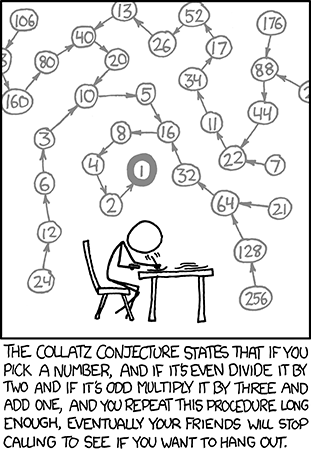
\includegraphics[scale=.5]{img/collatz_conjecture.png}
    \end{figure}
    (xkcd)
\end{frame}

\backupend

\end{document}
